\documentclass[conference]{IEEEtran}
\RequirePackage{cite}
\RequirePackage{amsmath,amssymb,amsfonts}
\RequirePackage{algorithmic}
\RequirePackage{graphicx}
\RequirePackage{textcomp}
\RequirePackage{xcolor}
\RequirePackage{hyperref}
\RequirePackage{csquotes}
\setkeys{Gin}{width=0.4\textwidth}
\def\BibTeX{{\rm B\kern-.05em{\sc i\kern-.025em b}\kern-.08em
    T\kern-.1667em\lower.7ex\hbox{E}\kern-.125emX}}
\begin{document}
\title{EECS 106B Final Project Proposal}
\author{Andrew~Fearing, Neelay~Junnarkar,  Hamza~Kamran~Khawaja}
\maketitle


\begin{abstract}
We will develop a robust control scheme for underactuated USV's.
\end{abstract}


\section{About Us}
Neelay is a 4th year undergraduate in EECS, and has taken courses such as EE 128, 221A/222, and (of course) EECS 106A. His interests are primarily related to control and motion planning.

Andrew is a 4th year undergraduate in EECS. He has taken EE 120, EE C128, and EECS C106A. His interests in robotics are in micro-scale mobile robots.
\section{Research Question}
Can we control a boat so that it keeps its lane? Autonomously navigate a canal.
\section{Motivation}
Boat stuck.
\begin{figure}
    \centering
    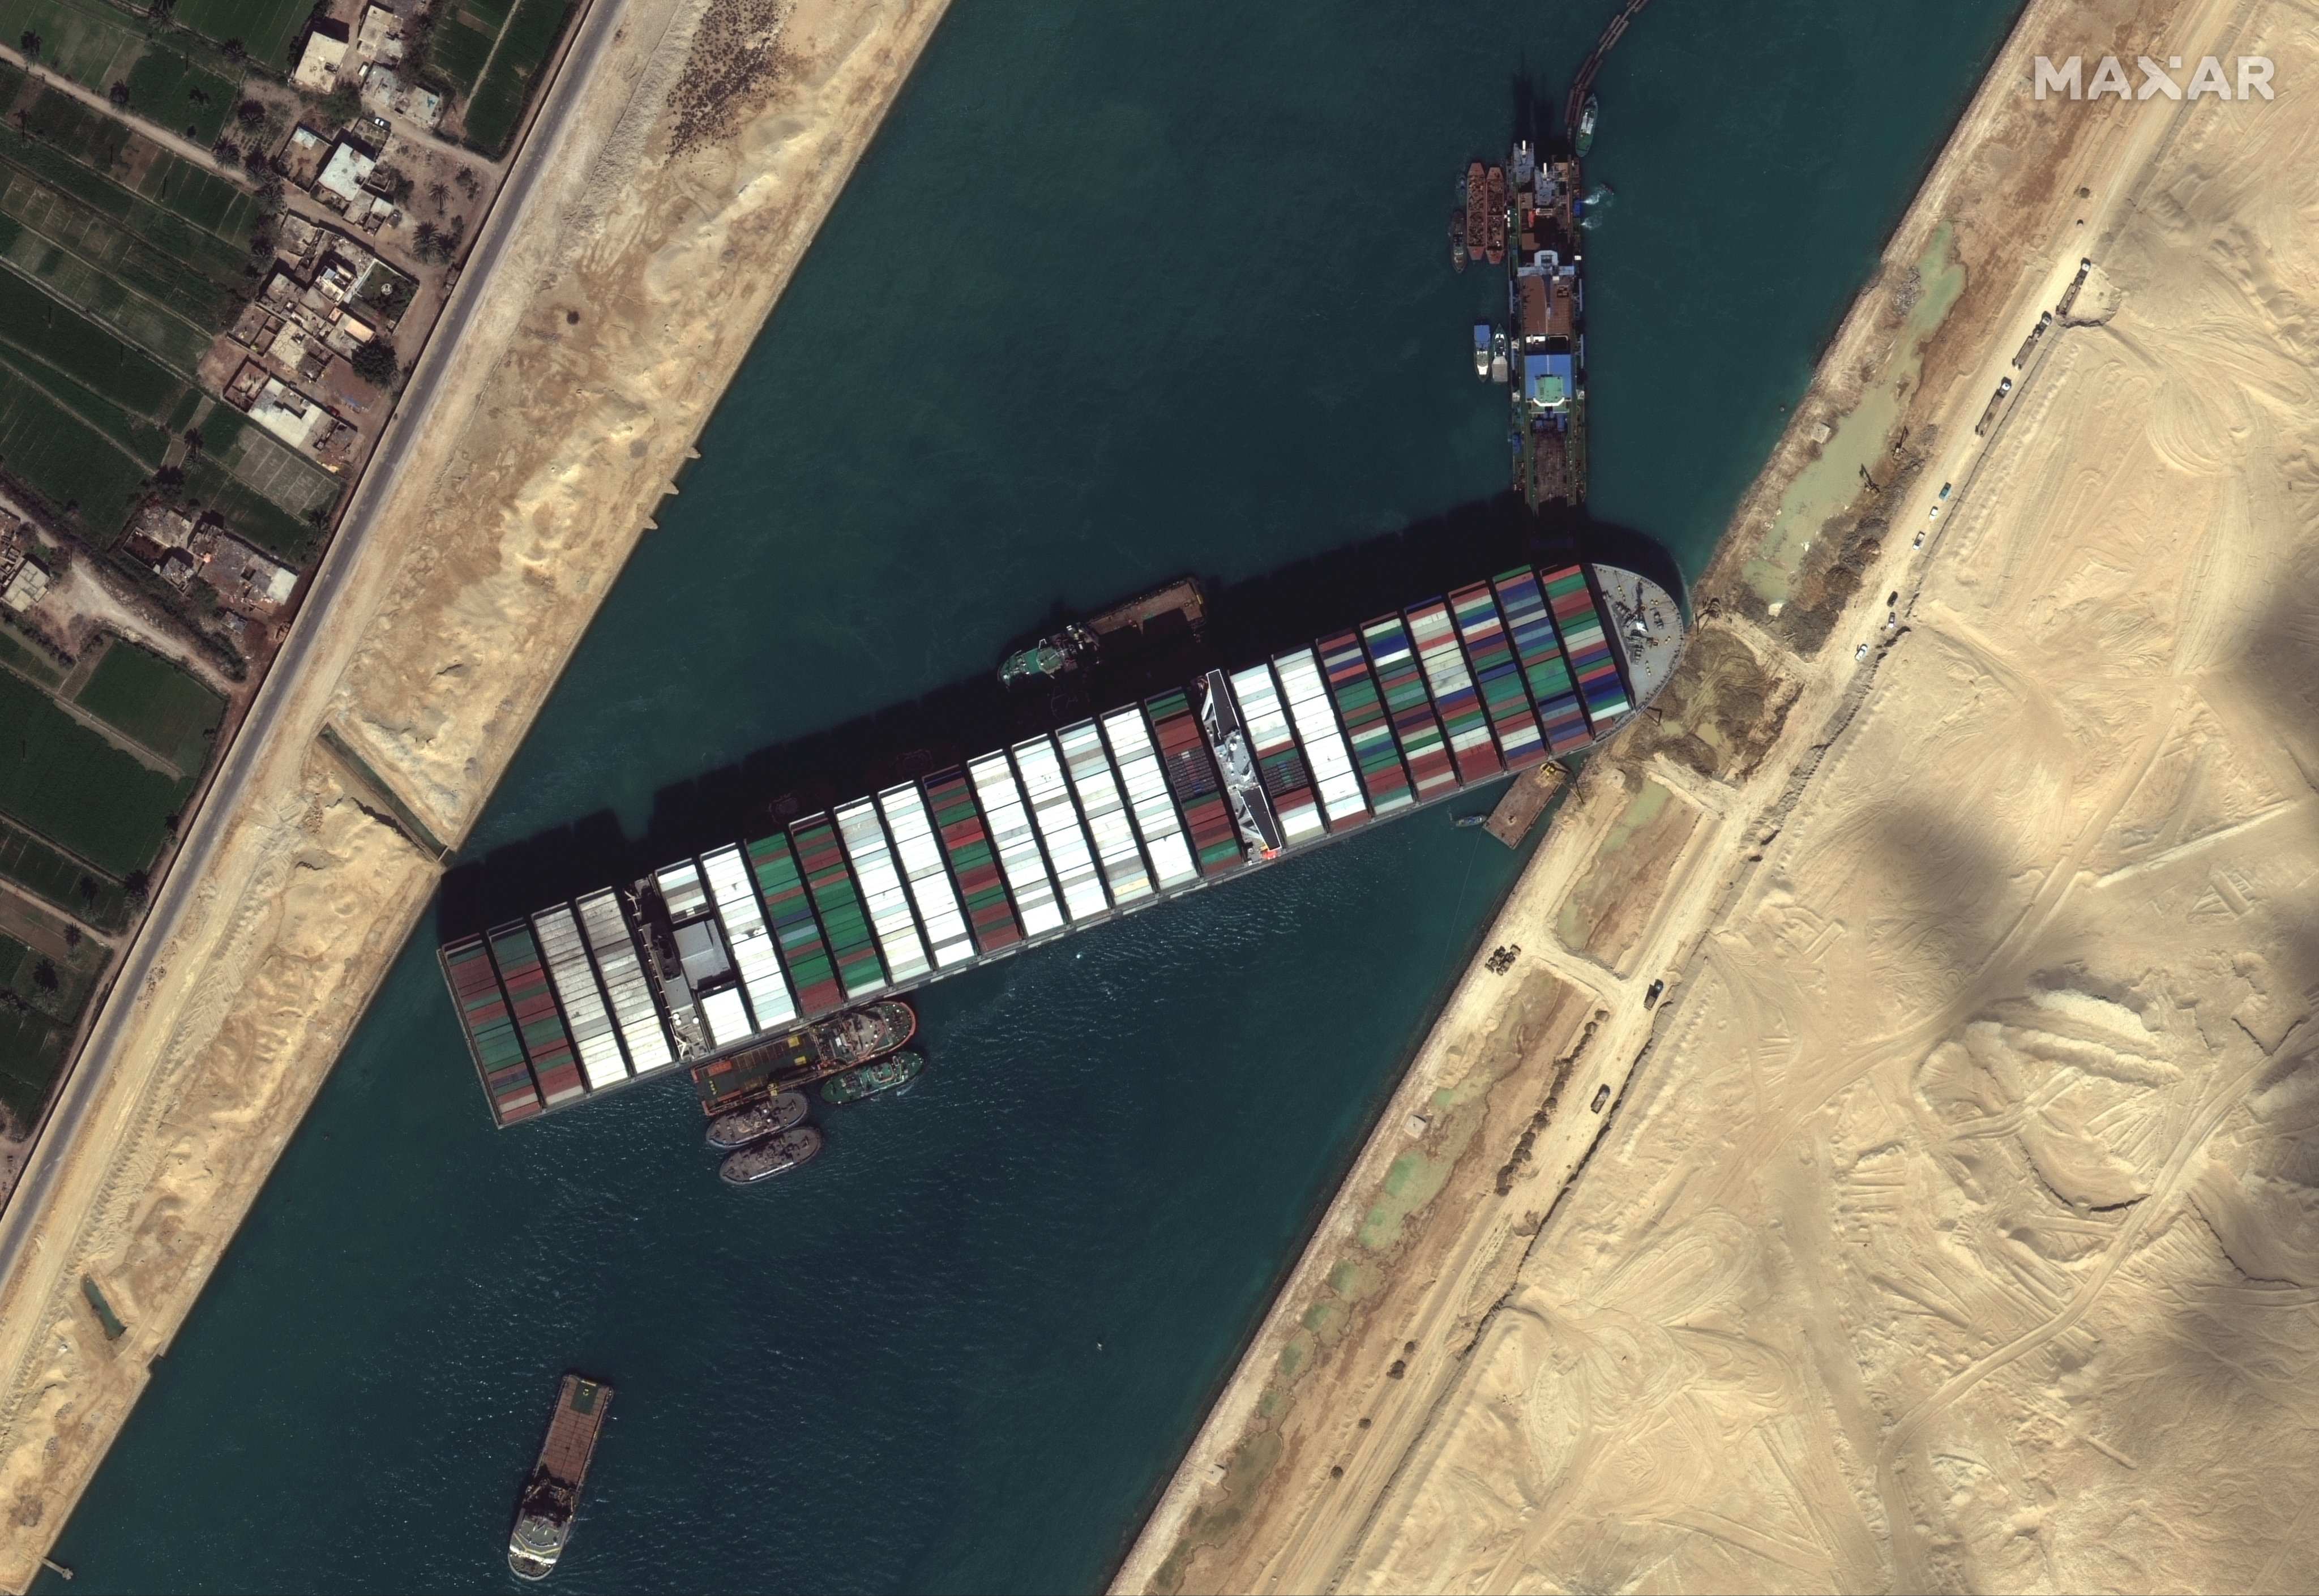
\includegraphics{documents/proposal/Suez_Canal_blocked_by_Ever_Given_March_27_2021.jpg}
    \caption{Boat stuck\label{fig:boat_stuck}}
\end{figure}
Control and safety of automobiles is an area of intense research focus. We want to try applying the same techniques to a different system: autonomous boats, or in engineering terms, \enquote{Unmanned Surface Vehicles}.
\section{Proposed Methodology}
We plan to use simulation to quantify the performance of our control scheme. We will examine literature in USV's.
\section{Related Work}
There is already work in the area of of USV's.

\cite{Setiawan2020} and \cite{Buehler2018} develop a dynamic models of an autonomous sailboats, though they do not go into the application of controls.

We hope to incorporate the control barrier functions we learned about in our presentation on \cite{Ames2019} to provide robustness.


\section{Experimental Plan}
Using a dynamic model as that proposed in \cite{Buehler2018}, we will simulate and analyze the performance of our control scheme.

\bibliographystyle{IEEEtran}
\bibliography{refs.bib}
\end{document}